\documentclass[a4paper, UTF-8]{article}
\usepackage{algorithm}
\usepackage{algpseudocode}
\usepackage{amsmath}
\usepackage{amsfonts}
\usepackage{amsthm}
\usepackage{tikz}
\usetikzlibrary{automata, positioning, arrows, trees}
\usepackage[utf8]{inputenc} % allow utf-8 input
\usepackage[T1]{fontenc}    % use 8-bit T1 fonts
\usepackage{hyperref}       % hyperlinks
\usepackage{url}            % simple URL typesetting
\usepackage{booktabs}       % professional-quality tables
\usepackage{amsfonts}       % blackboard math symbols
\usepackage{nicefrac}       % compact symbols for 1/2, etc.
\usepackage{microtype}      % microtypography
\usepackage{xcolor}         % colors

\theoremstyle{plain}
\newtheorem{theorem}{\indent Theorem}[section]
\newtheorem{lemma}[theorem]{\indent Lemma}
\newtheorem{assumption}{\indent Assumption}[section]
\newtheorem{note}[theorem]{\indent Notation}
\newtheorem{proposition}[theorem]{\indent Proposition}
\newtheorem{corollary}[theorem]{\indent Corollary}
\newtheorem{definition}{\indent Definition}[section]
\newtheorem{example}{\indent Example}[section]
\newtheorem{remark}{\indent Remark}[section]
\newenvironment{solution}{\begin{proof}[\indent\bf Solution]}{\end{proof}}
\renewcommand{\proofname}{\indent\bf Proof}

\begin{document}

\title{\bf{Lab7 Answers}}

\author{Yanqiao Chen*\\ 
  Department of Computer Science and Engineering\\
  Southern University of Science and Technology\\
  \texttt{12412115@mail.sustech.edu.cn}
  }

\maketitle

\section{Question 1} 

\begin{proof} 

Informally, the PDA may first read $a^*b^*$, and push $a$ in the first stack, $b$ in the second stack. Then every time it reads $c$, it pops one $a$ and one $b$. Finally, if the input is empty and both stacks are empty, the PDA accepts the input. If one stack is empty but the other is not, i.e., it reads one $\mathdollar$ and an $a$ or $b$ from the top of the stacks, the PDA will not accept the input. If both stacks are not empty at the end of the input, the PDA will also not accept the input.

\end{proof}

\section{Question 2}

\subsection{a)} 

\begin{enumerate}
    \item $q_10$ 
    \item $\sqcup q_2$
    \item $\sqcup \sqcup q_{accept}$
\end{enumerate}

\subsection{b)} 

\begin{enumerate}
    \item $q_100$ 
    \item $\sqcup q_20$
    \item $\sqcup x q_{3}$
    \item $\sqcup q_5 x$ 
    \item $q_5 \sqcup x$
    \item $\sqcup q_2 x$ 
    \item $\sqcup x q_2$ 
    \item $\sqcup x \sqcup q_{accept}$
\end{enumerate}

\subsection{c)} 

\begin{enumerate}
    \item $q_1000$ 
    \item $\sqcup q_2 00$ 
    \item $\sqcup x q_3 0$ 
    \item $\sqcup x 0 q_4$ 
    \item $\sqcup x 0 \sqcup q_{reject}$
\end{enumerate}

\subsection{d)} 

\begin{enumerate}
    \item $q_1000000$ 
    \item $\sqcup q_2 000000$ 
    \item $\sqcup x q_3 00000$
    \item $\sqcup x 0 q_4 0000$
    \item $\sqcup x 0 x q_3 000$
    \item $\sqcup x 0 x 0 q_400$
    \item $\sqcup x 0 x 0 x q_30$
    \item $\sqcup x 0 x 0 x 0 q_4 $
    \item $\sqcup x 0 x 0 x 0 \sqcup q_{reject}$
\end{enumerate}

\section{Question 3} 

\begin{itemize}
    \item [a.] Yes. The blank symbol $\sqcup$ is in the tape alphabet $\Gamma$, and the Turing machine can write $\sqcup$ on the tape. 
    \item [b.] No. The input alphabet $\Sigma$ does not contain the blank symbol $\sqcup$, thus the tape alphabet $\Gamma$ cannot be the same as $\Sigma$.
    \item [c.] No. The transition function $\delta$ is defined as $\delta: Q \times \Gamma \rightarrow Q \times \Gamma \times \{L, R\}$, which means that the head must move left or right after each transition, thus it cannot stay in the same position.
    \item [d.] No. The Turing machine must have at least one accepting state and at least one rejecting state, thus it cannot have only one state.
\end{itemize}

\section{Question 4}

The TM scans left-to-right, matching one $a$, one $b$, and one $c$ on each pass.
Symbols are marked with $X,Y,Z$ to indicate they have been counted.
All transitions not shown go to $q_{\text{reject}}$.

\begin{center}
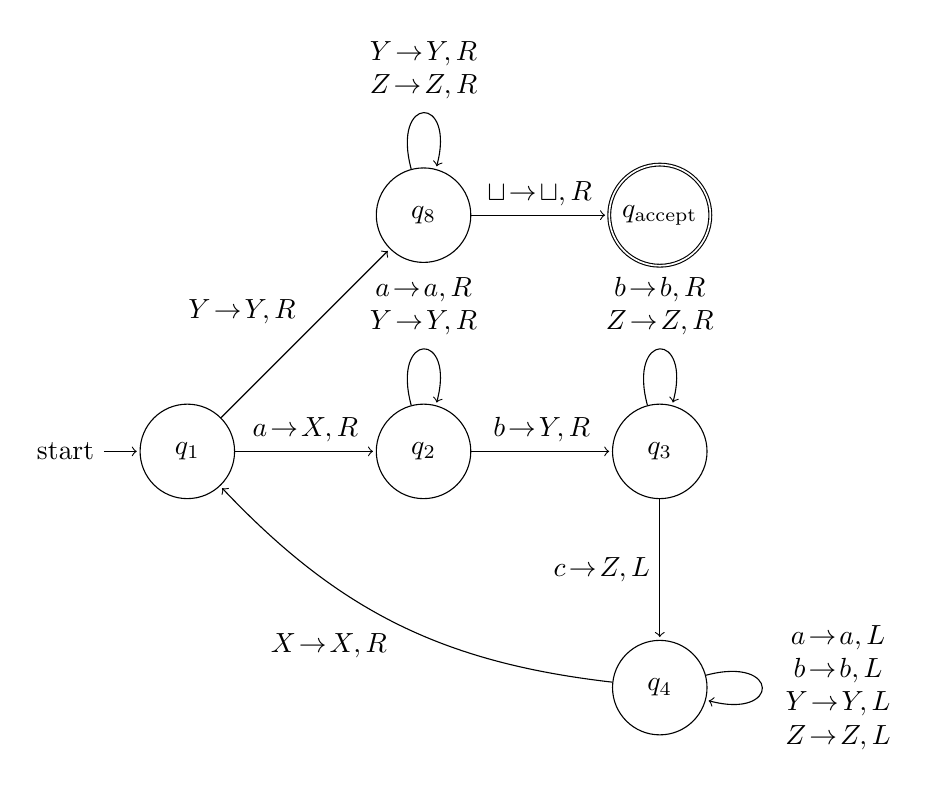
\begin{tikzpicture}[shorten >=1pt,node distance=3cm,on grid,auto, every state/.style={minimum size=1.2cm}]
    \node[state,initial]   (q1) {$q_1$};
    \node[state]           (q2) [right=of q1] {$q_2$};
    \node[state]           (q3) [right=of q2] {$q_3$};
    \node[state]           (q4) [below=of q3] {$q_4$};
    \node[state]           (q8) [above=of q2] {$q_8$};
    \node[state,accepting] (qa) [right=of q8] {$q_{\text{accept}}$};

    \path[->]
        (q1) edge node {$a\!\to\!X,R$} (q2)
             edge node[above left] {$Y\!\to\!Y,R$} (q8)
        (q2) edge[loop above] node {$\begin{array}{c}a\!\to\!a,R\\Y\!\to\!Y,R\end{array}$} (q2)
             edge node {$b\!\to\!Y,R$} (q3)
        (q3) edge[loop above] node {$\begin{array}{c}b\!\to\!b,R\\Z\!\to\!Z,R\end{array}$} (q3)
             edge node[left] {$c\!\to\!Z,L$} (q4)
        (q4) edge[loop right] node {$\begin{array}{c}a\!\to\!a,L\\b\!\to\!b,L\\Y\!\to\!Y,L\\Z\!\to\!Z,L\end{array}$} (q4)
             edge[bend left=20] node[below left] {$X\!\to\!X,R$} (q1)
        (q8) edge[loop above] node {$\begin{array}{c}Y\!\to\!Y,R\\Z\!\to\!Z,R\end{array}$} (q8)
             edge node {$\sqcup\!\to\!\sqcup,R$} (qa);
\end{tikzpicture}
\end{center}

\section{Question 5}

\subsection{a)}

On input $w$ over $\{0,1\}$:
\begin{itemize}
    \item Scan the tape. If no unmarked $0$ or $1$ remains, \emph{accept}.
    \item Find the leftmost unmarked $0$ and mark it with $X$.
    \item Continue scanning right and find the leftmost unmarked $1$; mark it with $X$.
    \item If a matching $1$ cannot be found, \emph{reject}.
    \item Return the head to the leftmost unmarked symbol and repeat.
\end{itemize}
Each iteration cancels one $0$ with one $1$, so the machine accepts exactly when their counts are equal.

\subsection{b)}

On input $w$ over $\{0,1\}$:
\begin{itemize}
    \item Scan the tape. If no unmarked symbols remain, \emph{accept}.
    \item Find the leftmost unmarked $1$ and mark it with $X$.
    \item Scan right to find the first unmarked $0$ and mark it with $X$; then find a second unmarked $0$ and mark it with $X$.
    \item If two matching $0$'s cannot be found, \emph{reject}.
    \item Return the head to the leftmost unmarked symbol and repeat.
\end{itemize}
Each iteration consumes one $1$ and two $0$'s, so the machine accepts exactly when $\#0 = 2\cdot\#1$.

\subsection{c)}

This is the complement of the language in part~(b). Since Turing machines are closed under complement for \emph{decidable} languages, construct a TM $M'$ that runs the decider $M$ from part~(b) and then flips the answer:
\begin{itemize}
    \item Run $M$ on $w$.
    \item If $M$ accepts, $M'$ \emph{rejects}; if $M$ rejects, $M'$ \emph{accepts}.
\end{itemize}
Thus $M'$ decides $\{w \mid w \text{ does not contain twice as many 0s as 1s}\}$. 

\section{Question 6} 

\begin{proof}

Any Turing machine can simulate a Turing machine with left reset, thus Turing Machines $\Leftarrow$ Turing Machines with left reset. We then show the opposite direction, i.e., Turing Machines $\Rightarrow$ Turing Machines with left reset.

We use the extended alphabet $\Gamma' = \Gamma \times \{0, 1, 2\}$ and state with $Q' = Q \times \{normal, clear\}$. 

When we want to reset, we denote the symbol with $2$, i.e., $c^2$. Then we turn to the leftmost symbol and change it into $a^1$. Then we follow the cycles: 
\begin{itemize}
    \item Reset and read until we meet a symbol with $1$, read the next one, if it is denote with $2$, change it into $0$.
    \item If it is denote with $0$, change it into $1$ and reset with state changing into the clearing state. 
    \item We continue to read until we meet a symbol with $1$, change it into $0$ and reset with normal mode. 
    \item Repeat. 
\end{itemize}

After this, the left one is the symbol with $1$, and the right one is the symbol with $2$. Then we stop at the leftmost symbol with notation $1$ and change it into $0$. Then the operation is equivalent to the original Turing machine with left shift.

\begin{example}
On the tape 
$$
abba
$$
and we are at the end. We first denote the symbol with $2$, i.e.,
$$
abba^2
$$

For simplicity, we only explicitly write out symbol with $1$ and $2$.

Then we turn to the leftmost symbol and change it into $a^1$, i.e., $a^1bba^2$, then we follow the cycles:
\begin{enumerate}
    \item We find the symbol with $1$ and read the next one, which is $b^0$, we change it into $b^1$ and reset with state changing into the clearing state, i.e., $a^1b^1ba^2$.
    \item We find the symbol with $1$ and change it into $0$, i.e., $ab^1ba^2$, and reset with normal mode.
    \item We find the symbol with $1$ and read the next one, which is $b^0$, we change it into $b^1$ and reset with state changing into the clearing state, i.e., $ab^1b^1a^2$.
    \item We find the symbol with $1$ and change it into $0$, i.e., $abb^1a$, and reset with normal mode.
    \item We find the symbol with $1$ and read the next one, which is $a^2$, we change it and stop. Then we reset and read the symbol with $1$, i.e., $abb^1a$, when we read it, we do the operation after the left shift in the original Turing machine and our head is on the third $b$, which is equivalent to the original Turing machine with left shift.
\end{enumerate}

For any $\delta(q, a) = (q', b, L)$, we may use the operation above to simulate it, and the last step will be $\delta(q, a^1) = (q', b^0, D)$, where $D$ denotes an head operation. 

\end{example}

The Turing machine with left reset can simulate any Turing machine, thus Turing Machines $\Rightarrow$ Turing Machines with left reset.

This means that Turing Machines $\Leftrightarrow$ Turing Machines with left reset, thus it can recognize all the Turing-recognizable languages.

\end{proof}

\section{Question 7} 

\begin{theorem}
    A Turing machine whose transition function uses only \emph{Right} (\texttt{R}) and \emph{Stay} (\texttt{S}) operations recognizes exactly the class of regular languages.
\end{theorem}

\begin{proof}
    Let $M = (Q, \Sigma, \Gamma, \delta, q_0, q_{\text{accept}}, q_{\text{reject}})$ be a Turing machine whose transition function is of the form
    \[
        \delta \colon Q \times \Gamma \longrightarrow Q \times \Gamma \times \{R, S\}.
    \]
    We construct a DFA $D = (Q_D, \Sigma, \delta_D, q_{\text{start}}, F_D)$ such that $L(D) = L(M)$.

    \paragraph{Observation.}
    Since $M$ is never allowed to move its head left, any symbol written on a tape cell at position $i$ will never be read again after the head leaves position $i$. Consequently, the only effect of a sequence of $S$-transitions on the same cell is the state $M$ is in when it finally executes an $R$-transition.

    \paragraph{State set.}
    The states of $D$ are drawn from $Q$ together with a trap state:
    \[
        Q_D \;=\; Q \cup \{\,q_{\text{dead}}\,\}.
    \]

    \paragraph{Transition function $\delta_D$.}
    Fix a state $q \in Q$ and an input symbol $a \in \Sigma$.
    Starting from the configuration in which $M$ is in state $q$ and reading $a$ on the tape,
    repeatedly apply transitions of the form $\delta(\cdot, \cdot) = (\cdot, \cdot, S)$.
    There are two possibilities:
    \begin{enumerate}
        \item[(i)] The machine eventually applies a transition with $R$; let $p \in Q$ be the state entered immediately after that $R$.  Define
            \[
                \delta_D(q, a) \;:=\; p.
            \]
        \item[(ii)] The machine never applies an $R$-transition; it either loops forever through $S$-transitions or halts in $q_{\text{reject}}$.  Define
            \[
                \delta_D(q, a) \;:=\; q_{\text{dead}}.
            \]
    \end{enumerate}
    Finally, set $\delta_D(q_{\text{dead}}, a) := q_{\text{dead}}$ for all $a \in \Sigma$.

    \paragraph{Start state.}
    The initial state of $M$ need not itself be a state from which $M$ executes $R$.
    To handle the prefix of the computation before the first $R$-transition, define
    \[
        q_{\text{start}} \;:=\;
        \begin{cases}
            p & \text{if starting from }(q_0, \sqcup)\text{ the first }R\text{-transition leads to }p \in Q,\\
            q_{\text{dead}} & \text{otherwise.}
        \end{cases}
    \]
    (More symmetrically, one may augment the input with a left-endmarker and treat the initial move from $\sqcup$ uniformly.)

    \paragraph{Accepting states.}
    Once the input has been consumed, $M$ reads blank symbols $\sqcup$ to the right of the input.  It is in these post-input $S/R$ cycles that $M$ decides acceptance.  Hence define
    \[
        F_D \;=\; \{\, q \in Q \mid \text{starting from configuration }(q, \sqcup),\; M\text{ eventually enters }q_{\text{accept}} \,\}.
    \]

    \paragraph{Correctness.}
    We argue by induction on the tape position $i \geq 1$ that after reading the first $i$ input symbols, $D$ is in exactly the state $M$ occupies immediately after the $R$-transition that moves its head from cell $i$ to cell $i+1$.  The base case ($i=0$) holds by definition of $q_{\text{start}}$; the inductive step follows from the definition of $\delta_D$.  When the input is exhausted, $D$ is in the state $M$ would be in upon first reading $\sqcup$ after the last input symbol.  By construction, this state lies in $F_D$ iff $M$ accepts.

    Therefore $L(D) = L(M)$, and $M$ recognizes a regular language.
\end{proof}

Thus the machine is not equivalent to a Turing machine, and it cannot recognize all the Turing-recognizable languages. It can only recognize regular languages.

\section{Question 8} 

\subsection{a)} 

Constructing a new start state with 2 $\epsilon$-transition to the two original start state. Thus the new NTM can simulate both of the original NTMs, and it accepts if either of the original NTMs accepts. It reject if both of the original NTMs reject.

\subsection{b)} 

Constructing a new $\epsilon$-transition from the accepting state of the first NTM to the start state of the second NTM. Thus the new NTM can simulate any concatenation of the string in the language of the two original NTMs, and it accepts if it reach the accepting state. It reject if it reach the rejecting state of the first NTM, or all the computing branches reach the rejecting state of the second NTM after simulating the first NTM.

\subsection{c)} 

Constructing a new start state pointing to the original start state with $\epsilon$-transition, and constructing a new $\epsilon$-transition from the accepting state to the start state. Thus the new NTM can simulate any repetition of the string in the language of the original NTM, and it accepts if it reach the accepting state. It reject if all the computing branches reach the rejecting state of the original NTM.

\subsection{d)} 

Let a NTM simulate the original NTM, and if it accepts, the new machine rejects; if it rejects, the new machine accepts. Thus the new NTM can simulate the original NTM, and it accepts if the original NTM rejects. It reject if the original NTM accepts. The new NTM can recognize the complement of the language recognized by the original NTM.

\subsection{e)} 

Let a NTM simulate have a two copy of the input string, and it simulates the original NTM on both of the copy. Let the workspace of the two simulation be separated. Thus the new NTM can simulate the original NTM on both copy of the input string, and it accepts if both of the simulation accepts. It reject if either of the simulation rejects. The new NTM can recognize the intersection of the language recognized by the original NTM.

\section{Question 9}

\begin{proof}
Let $L_1$ and $L_2$ be two Turing-recognizable languages, and let $M_1$ and $M_2$ be TMs that recognize them, respectively.

\paragraph{a. Union.}
Construct a TM $M$ that on input $w$ runs $M_1$ and $M_2$ on $w$ in parallel (using dovetailing). If $M_1$ accepts, $M$ \emph{accepts}; if $M_2$ accepts, $M$ \emph{accepts}. If $w \in L_1 \cup L_2$, at least one of the two machines accepts, so $M$ accepts. Hence $L_1 \cup L_2$ is Turing-recognizable.

\paragraph{b. Concatenation.}
Construct a TM $M$ that on input $w$ nondeterministically guesses a split $w = uv$. It then runs $M_1$ on $u$ and $M_2$ on $v$. If both accept, $M$ \emph{accepts}. If $w \in L_1 L_2$, there exists at least one split on which both machines accept, so $M$ accepts. Thus $L_1 L_2$ is Turing-recognizable.

\paragraph{c. Star.}
Construct a TM $M$ that on input $w$ first \emph{accepts} if $w = \varepsilon$. Otherwise it nondeterministically guesses a decomposition $w = w_1 w_2 \cdots w_k$ with $k \ge 1$ and each $w_i \neq \varepsilon$, and runs $M_1$ on each piece. If every run accepts, $M$ \emph{accepts}. This shows $L_1^*$ is Turing-recognizable.
\end{proof}

\section{Question 10} 

\subsection{a)}

On input $x$ (a positive binary number with the least significant bit on the right):
\begin{itemize}
    \item Move to the rightmost bit.
    \item If it is $1$, change it to $0$ and halt.
    \item If it is $0$, change it to $1$ and move left; repeat moving left until finding the first $1$, change it to $0$, and halt.
\end{itemize}
This implements binary subtraction-by-one with borrowing.

\subsection{b)}

Assume the input is of the form $x \# y$. The TM computes $x - y$ as follows:
\begin{itemize}
    \item \emph{Loop:} Scan to the least significant bit of $y$.
    \item If all bits of $y$ are $0$ (i.e., $y$ has been reduced to zero), erase $y$ and the delimiter $\#$, compact the tape, and halt.
    \item Otherwise, apply the subroutine from part (a) to decrement $y$ by one.
    \item Then apply the same subroutine to decrement $x$ by one.
    \item Return to the start of the loop.
\end{itemize}
Since each iteration decrements both numbers by one, after exactly $y$ iterations $y$ becomes $0$ and $x$ has been reduced to $x - y$.

\subsection{c)}

Assume the input is $x \# y$ with $x > y$. The TM computes the quotient $q = \lfloor x / y \rfloor$ as follows:
\begin{itemize}
    \item Maintain a quotient area $q$ on the tape, initially $0$.
    \item Repeatedly subtract $y$ from the current $x$ using the procedure of part (b).
    \item Each time the subtraction succeeds, increment $q$ by one: scan to the least significant bit of $q$; flip trailing $1$'s to $0$ and the first $0$ to $1$; if all bits were $1$, append a new most significant $1$.
    \item If a subtraction fails because $x < y$, erase $x$, $y$, and the delimiter, leaving only $q$, and halt.
\end{itemize}
The loop executes exactly $\lfloor x / y \rfloor$ times, so the final $q$ equals the integer quotient.

\section{Question 11} 



\end{document}